\documentclass[tikz,border=6pt]{standalone}

\usepackage{amsmath}
\usepackage{sansmath}
\usepackage{xcolor}
\usetikzlibrary{arrows.meta}

\definecolor{coltreat}{HTML}{0066CC}
\definecolor{colout}{HTML}{D62828}
\definecolor{collatent}{HTML}{A6A6A6}
\definecolor{filllatent}{HTML}{F2F2F2}

\begin{document}
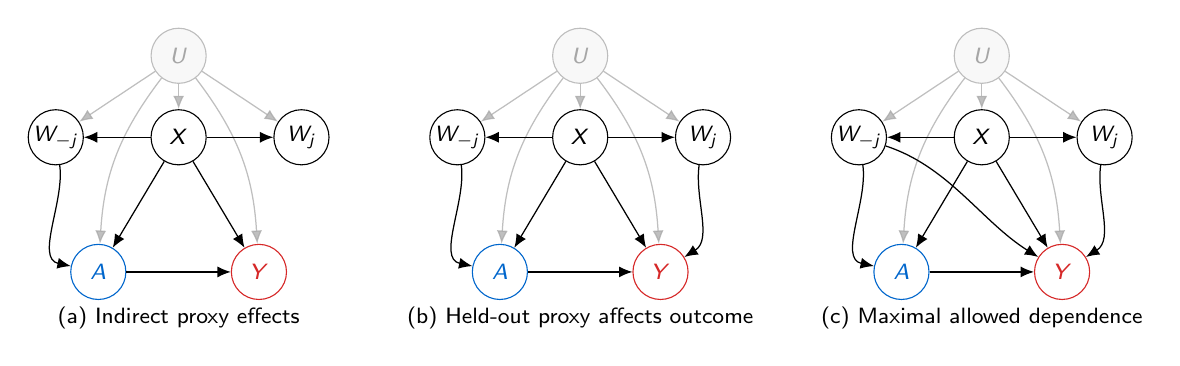
\begin{tikzpicture}[
  x=1.2cm,
  y=0.9cm,
  >={Latex[width=1.4mm,length=1.7mm]},
  font=\sffamily\sansmath\scriptsize,
  varnode/.style={draw,circle,inner sep=0mm,minimum size=7mm,
    font=\sffamily\sansmath\footnotesize},
  observed/.style={varnode,draw=black,text=black,fill=white},
  latent/.style={varnode,draw=collatent,draw opacity=0.72,text=collatent,
    fill=filllatent,fill opacity=0.55,text opacity=1},
  treatment/.style={varnode,draw=coltreat,text=coltreat,fill=white},
  outcome/.style={varnode,draw=colout,text=colout,fill=white},
  observed edge/.style={->,draw=black,line width=0.45pt},
  latent edge/.style={->,draw=collatent,opacity=0.72,line width=0.45pt}
]

% Panel (a): the smallest graph in the nested sequence.
\begin{scope}[xshift=0cm]
  \node[latent] (Ua) at (0,2.70) {$U$};
  \node[observed] (Wma) at (-1.30,1.55) {$W_{-j}$};
  \node[observed] (Xa) at (0,1.55) {$X$};
  \node[observed] (Wja) at (1.30,1.55) {$W_j$};
  \node[treatment] (Aa) at (-0.85,-0.35) {$A$};
  \node[outcome] (Ya) at (0.85,-0.35) {$Y$};

  \draw[latent edge] (Ua) -- (Wma);
  \draw[latent edge] (Ua) -- (Xa);
  \draw[latent edge] (Ua) -- (Wja);
  \draw[latent edge] (Ua) to[bend right=17] (Aa);
  \draw[latent edge] (Ua) to[bend left=17] (Ya);
  \draw[observed edge] (Xa) -- (Wma);
  \draw[observed edge] (Xa) -- (Wja);
  \draw[observed edge] (Xa) -- (Aa);
  \draw[observed edge] (Xa) -- (Ya);
  \draw[observed edge] (Wma) to[out=-82,in=168,looseness=0.92] (Aa);
  \draw[observed edge] (Aa) -- (Ya);

  \node[align=center,font=\sffamily\sansmath\footnotesize] at (0,-1.00)
    {(a) Indirect proxy effects};
\end{scope}

% Panel (b): panel (a) plus the held-out-proxy effect on outcome.
\begin{scope}[xshift=5.1cm]
  \node[latent] (Ub) at (0,2.70) {$U$};
  \node[observed] (Wmb) at (-1.30,1.55) {$W_{-j}$};
  \node[observed] (Xb) at (0,1.55) {$X$};
  \node[observed] (Wjb) at (1.30,1.55) {$W_j$};
  \node[treatment] (Ab) at (-0.85,-0.35) {$A$};
  \node[outcome] (Yb) at (0.85,-0.35) {$Y$};

  \draw[latent edge] (Ub) -- (Wmb);
  \draw[latent edge] (Ub) -- (Xb);
  \draw[latent edge] (Ub) -- (Wjb);
  \draw[latent edge] (Ub) to[bend right=17] (Ab);
  \draw[latent edge] (Ub) to[bend left=17] (Yb);
  \draw[observed edge] (Xb) -- (Wmb);
  \draw[observed edge] (Xb) -- (Wjb);
  \draw[observed edge] (Xb) -- (Ab);
  \draw[observed edge] (Xb) -- (Yb);
  \draw[observed edge] (Wmb) to[out=-82,in=168,looseness=0.92] (Ab);
  \draw[observed edge] (Wjb) to[out=-98,in=32,looseness=0.92] (Yb);
  \draw[observed edge] (Ab) -- (Yb);

  \node[align=center,font=\sffamily\sansmath\footnotesize] at (0,-1.00)
    {(b) Held-out proxy affects outcome};
\end{scope}

% Panel (c): panel (b) plus the remaining-proxy effect on outcome.
\begin{scope}[xshift=10.2cm]
  \node[latent] (Uc) at (0,2.70) {$U$};
  \node[observed] (Wmc) at (-1.30,1.55) {$W_{-j}$};
  \node[observed] (Xc) at (0,1.55) {$X$};
  \node[observed] (Wjc) at (1.30,1.55) {$W_j$};
  \node[treatment] (Ac) at (-0.85,-0.35) {$A$};
  \node[outcome] (Yc) at (0.85,-0.35) {$Y$};

  \draw[latent edge] (Uc) -- (Wmc);
  \draw[latent edge] (Uc) -- (Xc);
  \draw[latent edge] (Uc) -- (Wjc);
  \draw[latent edge] (Uc) to[bend right=17] (Ac);
  \draw[latent edge] (Uc) to[bend left=17] (Yc);
  \draw[observed edge] (Xc) -- (Wmc);
  \draw[observed edge] (Xc) -- (Wjc);
  \draw[observed edge] (Xc) -- (Ac);
  \draw[observed edge] (Xc) -- (Yc);
  \draw[observed edge] (Wmc) to[out=-82,in=168,looseness=0.92] (Ac);
  \draw[observed edge] (Wmc) to[out=-18,in=148,looseness=0.90] (Yc);
  \draw[observed edge] (Wjc) to[out=-98,in=32,looseness=0.92] (Yc);
  \draw[observed edge] (Ac) -- (Yc);

  \node[align=center,font=\sffamily\sansmath\footnotesize] at (0,-1.00)
    {(c) Maximal allowed dependence};
\end{scope}

\end{tikzpicture}
\end{document}
